\documentclass[tikz,border=50mm]{standalone}
% !TeX program = luatex

%===This is the preambule I call in every file===

\usepackage{tikz}
\usepackage{xcolor}
\usepackage{pgfplots}
\usepackage{circuitikz}
\usepackage{tikz-3dplot}
\pgfplotsset{compat=newest}
\usetikzlibrary{arrows.meta, shapes.geometric, positioning, perspective, patterns.meta, decorations.pathreplacing, decorations.pathmorphing, decorations.markings, patterns, arrows.meta, shapes, shapes.geometric, decorations.text, angles, quotes,calc, 3d, math, circuits.ee.IEC,hobby, knots, intersections, through}


%=== The Euler Med Logo ===
%=== i.e. My signature ===

\usepackage{amsmath, amsfonts}
\makeatletter
\newcommand*\eulermed{{
\scalebox{3.3}{$\mathbb{E}$}\kern-1pt \scalebox{1.5}{u$\ell\varepsilon\rho$}\kern-55pt
\raisebox{19pt}{\scalebox{1.5}{$\mathcal{M}\varepsilon\delta$}}}
\@}
\makeatother

\begin{document}
\begin{document}
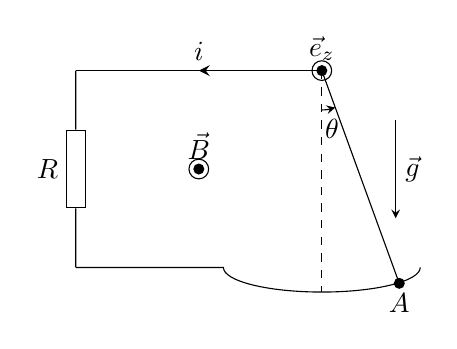
\begin{tikzpicture}[>=stealth,circuit ee IEC,scale=1.25]
\tikzstyle arrowstyle=[scale=1.25] 
\tikzstyle directed=[postaction={red,decorate,decoration={markings,mark=at position .5 with{\arrow[arrowstyle]{stealth}}}}]
\draw[directed] (0,0)--(-2.5,0) node[above, midway] {$i$};
\draw[] (-2.5,0)to[resistor] (-2.5,-2);
\node[left=0.1] at (-2.5,-1) {$R$};
\draw (-2.5,-2)--(-1,-2) arc (-180:0:1 and 0.25) (0,-2);
\draw[dashed] (0,0)--(0,-2.25);
\draw[fill=black] (0,0)--(-70:2.3)circle(0.05) node[below] {$A$};
\draw[->] (0.75,-0.5)--(0.75,-1.5) node[midway, right] {$\vec{g}$};
\draw[] (0,0)circle(0.1) node[above] {$\vec{e}_z$};
\filldraw[] (0,0)circle(0.05);
\draw[] (-1.25,-1)circle(0.1) node[above] {$\vec{B}$};
\filldraw[] (-1.25,-1)circle(0.05);
\coordinate(o) at (0,0);
\coordinate(a) at (-70:2.3);
\coordinate(g) at (0,-2.25);
 \pic[draw,->,inner sep=1pt,circle, draw,angle
eccentricity=1.5, "$\theta$", angle radius = 5mm] {angle = g--o--a};
\end{tikzpicture}
\end{document}
